\chapter{\IfLanguageName{dutch}{Stand van zaken}{State of the art}}%
\label{ch:stand-van-zaken}

% Tip: Begin elk hoofdstuk met een paragraaf inleiding die beschrijft hoe
% dit hoofdstuk past binnen het geheel van de bachelorproef. Geef in het
% bijzonder aan wat de link is met het vorige en volgende hoofdstuk.

% Pas na deze inleidende paragraaf komt de eerste sectiehoofding.

Dit hoofdstuk bevat je literatuurstudie. De inhoud gaat verder op de inleiding, maar zal het onderwerp van de bachelorproef *diepgaand* uitspitten.
De bedoeling is dat de lezer na lezing van dit hoofdstuk helemaal op de hoogte is van de huidige stand van zaken (state-of-the-art) in het onderzoeksdomein.
Iemand die niet vertrouwd is met het onderwerp, weet nu voldoende om de rest van het verhaal te kunnen volgen, zonder dat die er nog andere informatie moet over opzoeken \autocite{Pollefliet2011}.

Je verwijst bij elke bewering die je doet, vakterm die je introduceert, enz.\ naar je bronnen. In \LaTeX{} kan dat met het commando \texttt{$\backslash${textcite\{\}}} of \texttt{$\backslash${autocite\{\}}}. Als argument van het commando geef je de ``sleutel'' van een ``record'' in een bibliografische databank in het Bib\LaTeX{}-formaat (een tekstbestand). Als je expliciet naar de auteur verwijst in de zin (narratieve referentie), gebruik je \texttt{$\backslash${}textcite\{\}}. Soms is de auteursnaam niet expliciet een onderdeel van de zin, dan gebruik je \texttt{$\backslash${}autocite\{\}} (referentie tussen haakjes). Dit gebruik je bv.~bij een citaat, of om in het bijschrift van een overgenomen afbeelding, broncode, tabel, enz. te verwijzen naar de bron. In de volgende paragraaf een voorbeeld van elk.

\textcite{Knuth1998} schreef een van de standaardwerken over sorteer- en zoekalgoritmen. Experten zijn het erover eens dat cloud computing een interessante opportuniteit vormen, zowel voor gebruikers als voor dienstverleners op vlak van informatietechnologie~\autocite{Creeger2009}.

Let er ook op: het \texttt{cite}-commando voor de punt, dus binnen de zin. Je verwijst meteen naar een bron in de eerste zin die erop gebaseerd is, dus niet pas op het einde van een paragraaf.


\section{Inefficiënt documentmanagement en repetitie}
\label{sec:documentmanagement}

\subsection{Repetitie}
In een advocatenkantoor is het vanzelfsprekend dat er heel veel administratie aan bod komt. Denk maar aan het opstellen van dagvaardingen,
ingebrekestellingen, e-mails, aangetekende brieven en andere communicatie.

Natuurlijk dringt zich dit op dat deze taken veel tijd in beslag kunnen nemen. Naast een administratief spectrum gaat het ook over verdediging van cliënten, pleiten en ander rechtbankwerk.

Moest er daar dan nog extra repetitief bureauwerk aan te pas komen, kan dit een obstakel vormen naar productiviteit toe. Hiervoor onderstaande citatie ter illustratie:
\begin{displayquote}
	\textit{"How much time is spent in repetitive tasks in the workplace? Today the typical office worker spends 10\% of their time on manual data entry into business applications,
		such as the ERP system, CRM or spreadsheets. In total, they spend over 50\% of work time creating or updating documents, eg. PDFs, spreadsheets or word documents \autocite{Workfellow}."}
\end{displayquote}

Natuurlijk is dit een generieke citatie die handelt over PDFs, spreadsheets en dergelijke, maar ze is zeker ook toepasbaar in een advocatenkantoor.

Het komt er op neer dat repetitie een killer is voor productiviteit omdat het juist zoveel tijd in beslag neemt,
volgende citatie handelt over het aantal copy pastes van een gemiddelde administratieve medewerker:

\begin{displayquote}
	\begin{itemize}
		\item \emph {A typical office worker spends 3 hours working on spreadsheets each week, for example in Microsoft Excel or Google Sheets.}
		\item \emph {A typical office worker spends almost 2 1/2 hours in business communications or email applications, such as Outlook.}
		\item \emph {A typical office worker spends over 1 1/2 hours each week searching and organizing files, for example in the shared file service such as Sharepoint or Google Drive.}
		\item \emph {A typical office worker spends 1 1/2 hours each week copy-pasting or manually entering data into business applications, such as the ERP or CRM.} \autocite{Workfellow}
	\end{itemize}
\end{displayquote}

\subsection{Het managen van grote hoeveelheden documenten}
Doorheen de jaren wordt er een heel groot archief aan documenten opgebouwd.
Het doorzoeken en onderhouden van dit archief kan voor velen een grote uitdaging vormen en ook heel veel tijd in beslag nemen,
dit kan de productiviteit van een kantoor in het gedrang brengen en heel tijdrovend zijn, zeker als het archief inefficiënt is opgebouwd.

Het opzoeken van documenten in een archief is een mooi voorbeeld om te vergelijken tussen menselijke en machinale zoekmethodes.
Het opzoeken van data in een archief kan parallel gesteld worden met een zoekmachine. Volgende citatie schetst oppervlakkig het verschil tussen
menselijke en digitale methodes.

\begin{displayquote}
	Search engines have been with us for several decades as an integral part of our digital life.
	We are casually searching over billions of web pages to retrieve and share information from various resources.
	While humans are very good at conversational context and background knowledge which helps them to deal with intrinsic ambiguity of words,
	it may not be true in case of search engines, especially when it comes to out-of-the-vocabulary searches \autocite{MediumSemanticSearch}
\end{displayquote}

Het artikel handelt verder over semantische zoekmethodes en schetst een voorbeeld met een voorbeeld-dataset en een proof-of-concept in Python.

Zoekmachines gebruikten echter niet altijd een semantische methodiek:

\begin{displayquote}
	At first, search engines were lexical: the search engine looked for literal matches of the query words,
	without understanding of the query’s meaning and only returning links that contained the exact query. \autocite{MediumSemanticSearch}
\end{displayquote}

Lexicaal zoeken is vrij simpel te implementeren en is een vrij primitief concept. Semantisch zoeken is daarentegen wat complexer te integreren:

\begin{displayquote}
	On the other hand, “Semantic Search” can simplify query building, because it is supported by automated natural language processing programs
	i.e. using Latent Semantic Indexing — a concept that search engines use to discover how a keyword and content work together to mean the same thing. \autocite{MediumSemanticSearch}
\end{displayquote}

Wat heeft dit nu te maken met documentmanagement? Een zoekmachine is een polyvalente tool die ingezet kan worden op verschillende datasets. Dit kan ook een volledig archief zijn van
documenten in een advocatenkantoor. Het implementeren van een semantisch zoekalgoritme kan een oplossing bieden op het eerste subprobleem: inefficiënt zoeken in dit archief.

\begin{displayquote}
	In brief, LSI(Latent Semantic Index) does not require an exact match to return useful results.
	Where a plain keyword search will fail if there is no exact match,
	LSI will often return relevant documents that don’t contain the keyword at all. \autocite{MediumSemanticSearch}
\end{displayquote}

\section{obstakels in research van rechtszaken}
Bij een (oppervlakkige) verkennende audit bij advocatenkantoor Deltalex viel op dat er veel tijd wordt gespendeerd aan het opzoeken van dossiergerelateerde informatie. Denk hierbij maar aan
contactgegevens (ondernemingsnummer, adres, ...) van een cliënt, dossierdata, technische specificaties, enz.

Voor een advocaat kan dit een bijzonder lang en repetitief proces vormen indien manueel uitgevoerd. Gelukkig kunnen hier technieken zoals RAG (Retrieval-Augmented Generation) een grote hulp
bij bewijzen. RAG (Retrieval Augmented Generation) is een van de grootste use cases voor LLM's en is een framework dat de fundamentele trainingsdata van een Large Language Model
combineert met bestaande data in een database. Zodoende kan een model gegronde antwoorden geven, gebaseerd op betrouwbare en relevante informatie.

Een quote van Medium legt uit hoe RAG werkt in grote lijnen:

\begin{displayquote}
	A typical RAG process, as pictured below, has an LLM, a collection of enterprise documents, and supporting infrastructure to improve information retrieval and answer construction.
	The RAG pipeline looks at the database for concepts and data that seem similar to the question being asked, extracts the data from a vector database and reformulates the data into
	an answer that is tailored to the question asked. This makes RAG a powerful tool for companies looking to harness their existing data repositories for enhanced decision-making
	and information access. \autocite{MediumRAG}
	\begin{figure}[h]
		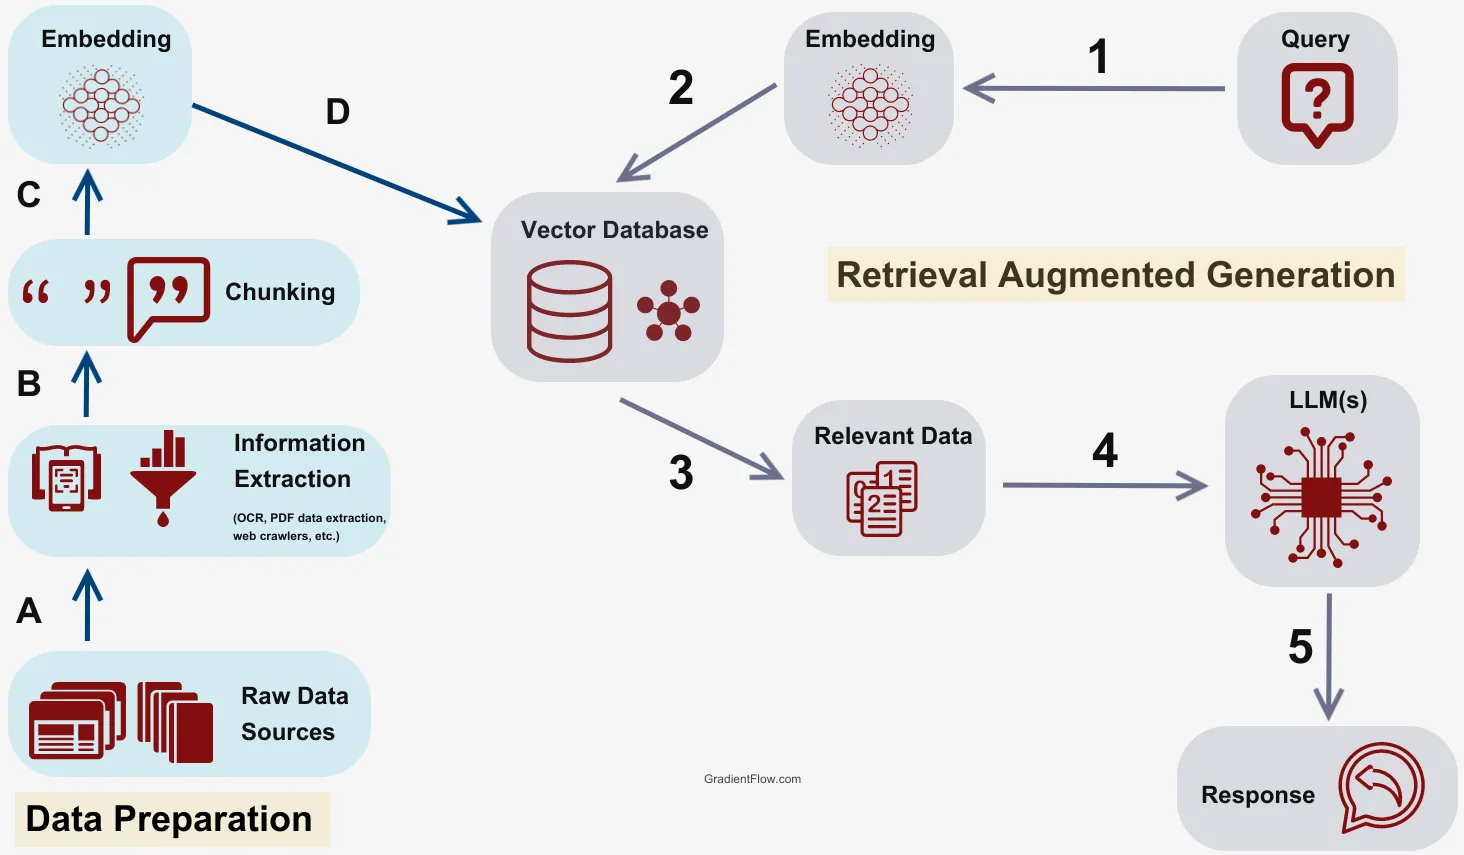
\includegraphics[width=\textwidth]{RAG.png}
		\centering
	\end{figure}
\end{displayquote}
\newpage

RAG kan hier dienst doen als een mogelijke plaatsvervanger voor manuele research en het opstellen van communicatiedocumenten (zoals aangetekende brieven, invorderingen, ...). Deze optie zal in
een later stadium van deze bachelorproef geëvealueerd worden. Advocatuur is een heel toepasselijk gebied voor RAG:

\begin{displayquote}
	Practically, RAG is likely preferable in environments like
	legal, customer service, and financial services where the ability to
	dynamically pull vast amounts of up-to-date data enables the most accurate and comprehensive responses.
\end{displayquote}

\section{Het automatiseren van administratieve taken}
Het manueel en persoonlijk afhandelen van 'simpele' administratieve taken door een advocaat zelf kan heel veel tijdverlies veroorzaken. Een digitale assistent kan bepaalde zaken
overnemen zoals het inplannen van consultaties, agendabeheer en routine		communicatie. In hoeverre kan een systeem dit overnemen? Is dit mogelijk?
De eerste dingen waar een ontwikkelaar van een dergelijke applicatie aan zou kunnen denken zijn zaken zoals hoe we een assistent toegang (lezen en schrijven) kunnen/ mogen geven tot
de persoonlijke agenda's van advocaten, programma's, ... Wat als er iets fout gaat en heel de agenda wordt overschreven met nutteloze data? Wat als afspraken bevestigd worden maar niet ingepland?

Het is ook niet echt ethisch verantwoord als een cliënt een som betaalt voor persoonlijke aandacht en communicatie en dan gegenereerde content voorgeschoteld krijgt.
Aan de andere kant kan het ook zijn dat een advocaat in tijdnood raakt en dat hij een snelle content boost ter zijn beschikking heeft.

Een LLM (dat ook gebruikt wordt voorgaande zaken) is hiervoor een ideale oplossing. Het kan dienen voor inspiratie of de generatie van een volledig document. Natuurlijk moet
een advocaat een persoonlijke behandeling verstrekken aan de cliënt dus deze optie wordt best alleen gebruikt in geval van nood.

Aan de andere kant kan een virtuele assistent wel instaan voor taken zoals agenda- en memobeheer.
Een dergelijke implementatie vereist integratie met bestaande software zoals Office365 (Microsoft) en ERP programma's en analyse van persoonlijke communicatie van een advocaat en zijn cliënt,
wat ons naadloos overbrengt naar de veiligheid van data tijdens het gebruik van digitale tools en digitale assistenten.

\section{Privacy en veiligheid  van data}
In advocatenkantoren wordt op een dagelijkse basis omgegaan met vertrouwelijke informatie van cliënten. Het is dan natuurlijk meer dan logisch dat de veiligheid van dergelijke informatie van
elementair belang is. Een citaat van "Legal buddies" staaft een paar protocollen om datasecurity en compliance met strikte dataregulaties zoals GDPR in de Europese Unie:

\begin{displayquote}
	Proper protocols must be implemented to keep sensitive case data protected and align usage to regional regulations.
	\begin{itemize}
		\item When working with legal AI systems, law firms must implement security controls like data encryption, access management, network segmentation, and intrusion detection.
		\item Usage and data sharing policies should conform to relevant privacy laws and professional ethics rules around legal data confidentiality.
		\item Firms can request third-party audits of AI provider security infrastructure for assurance on protection mechanisms.
		\item Using on-premise AI options instead of cloud-based ones may better align with internal compliance rules and risk tolerance levels.
		\item Regional laws may also dictate data residency and cross-border transfer restrictions. Understanding jurisdictional nuances allows appropriate legal AI adoption.
		\item Overall, prudent security and compliance positioning is vital for law firms exploring innovative technologies like AI-powered legal assistants. Partnering with trusted, vetted providers also reduces risk exposure.
	\end{itemize}

	With deliberate planning around privacy, ethics and regional legislation, firms can safely pursue AI efficiency gains.\autocite{LegalBuddies}
\end{displayquote}

Bij verdere research blijkt het grootste risico dat data van cliënten (onveilig) over het internet gestuurd wordt of dat de data blijft plakken op de cloud server van een externe tool.
De betere en veiligste optie blijkt hier om oftewel lokaal of in private cloud te hosten. In het hoofdstuk "Methodologie" zullen verschillende technologieën besproken worden om een dergelijke
setup te bereiken.

\section{Gebruiksgemak en aanpassing}
Een van de belangrijkste dingen in het inbrengen van nieuwe software in een bestaand kantoor is het gebruiksgemak en toegankelijkheid van de nieuwe programma's. Om deze zaken te garanderen,
moeten er een paar principes nauwlettend gevolgd worden. De beste manier om een design te krijgen waar de gebruiker centraal in staat is het verstaan van de requirements, pijnpunten en
workflows van advocaten. Dit is van elementair belang om een intuïtief systeem te bouwen dat naadloos integreert in hun workflow. Natuurlijk is dit niet het enige.
Laten we samen een paar belangrijke aspecten overlopen.

\subsection{Een intuïtieve interface}
De interface van een digitale assistent moet er overzichtelijk en netjes uitzien. Makkelijke navigatie is van elementair belang. Advocaten moeten snel en makkelijk de features kunnen aanspreken
zonder al te veel clutter en nutteloze toepassingen. De beste interface is er een die minimaal en ontworpen is met de gebruiker in het achterhoofd. Deze stelling kan onderbouwd worden met enkele
designprincipes uit een artikel van Zefort.com:

\begin{displayquote}
	\textbf{Simplicity and clarity:}
	By reducing complexity and providing clear instructions, legal services become more user-friendly and facilitate better access to justice for all.
	\autocite{Zefort}

	\textbf{Visual Hierarchy and Information Organization:}
	Prioritizing content through size, color, and contrast also aids in emphasizing key points and important details.
	\autocite{Zefort}

	\textbf{Clear and Accessible Navigation:}
	A well-designed navigation system helps lawyers, clients, and other users locate the information they need with minimal effort.
	\autocite{Zefort}
\end{displayquote}

\subsection{Natural language processing}
Om de leercurve van een digitale assistent te verlagen, moet hij in staat zijn om queries in natuurlijke taal te kunnen verwerken. 
Dit laat advocaten en medewerkers toe om de assistent te benaderen op dezelfde manier als een menselijke collega. Meer over NLP in het hoofdstuk methodologie. 

\subsection{Naadloze integratie}
Een dichte integratie met de bestaande software die gebruikt wordt is misschien wel één van de belangrijkste van de drie. Het succes van deze implementatie valt of staat met hoe makkelijk 
een advocaat ze kan integreren in hun bestaande workflow. Dit elimineert manuele invoer van manuele data of het constant switchen tussen verschillende applicaties. 

In conclusie: het succes van een digitale assistent (of in extensie bijna iedere digitale toepassing) hangt grotendeels af van de gebruikerservaring. 
Als je de voorgaande drie zaken zult prioriteren in de ontwikkeling van een tool, kun je makkelijker het volledige potentieel ervan bereiken en zodoende een kwalitatieve, nuttige tool leveren. 
